% !TEX encoding = UTF-8
% !TEX TS-program = pdflatex
% !TEX root = ../tesi.tex

%**************************************************************
\chapter{Progettazione}
\label{cap:progettazione}
In questo capitolo verrà trattato il secondo periodo del tirocinio: la progettazione e la codifica. Questa parte, avvenuta dopo l'Analisi dei Requisiti, è da ritenersi importante per il progetto in quanto ha occupato gran parte del tempo lavorativo. Il primo passo è stato eseguire la progettazione dell'architettura, in modo che i servizi necessari fossero correttamente configurati prima del loro effettivo utilizzo. Successivamente è stata eseguita la stesura del codice per la realizzazione della Skill. Nei paragrafi successivi seguiranno porzioni di codice significativo per la loro importanza e per il funzionamento di determinati servizi. Importante ricordare che il codice implementato e mostrato sarà in Node.js come quanto detto nel paragrafo \hyperref[nodejs]{1.4.1}. 
%**************************************************************
\section{Architettura}
Come riportato nel paragrafo \hyperref[serivizi-aws]{1.4.3}, il progetto si basa interamente sui servizi offerti dall'ecosistema Amazon. Di conseguenza è risultato facile ed immediato impostare i servizi dell'architettura in modo da rendere il tutto efficacie ed efficiente. In questo paragrafo si andrà a spiegare cosa offre ogni singolo servizio di AWS e come esso è stato impostato per il suo corretto funzionamento nella Skill.

\section{Configurazione servizi Amazon Web Service}
\subsection{AWS SES}
Amazon SES\footnote{AWS SES. URL: \href{https://aws.amazon.com/it/ses/}{https://aws.amazon.com/it/ses/}} (Simple Email Service) è un servizio di invio e-mail basato sul cloud messo a disposizione da Amazon per gli sviluppatori di applicazioni. Tale servizio è da considerarsi vantaggioso in quanto è affidabile e a costo ridotto, utile per qualunque tipo di azienda ed ideale per la realizzazione del progetto.
\newpage
\noindent Per utilizzare AWS SES è necessario impostare il servizio visitando la pagina\footnote{AWS SES. URL: \href{https://aws.amazon.com/it/ses/}{https://aws.amazon.com/it/ses/}} dedicata ed eseguire le istruzioni riportate:
\\[0.5cm]
\begin{minipage}{0.5\textwidth}
	\begin{figure}[H]
		
\includegraphics[width=6cm]{immagini/ses.png}
		\caption{\label{fig:icona_aws_ses}Icona AWS SES}
	\end{figure}
\end{minipage}
\begin{minipage}{0.5\textwidth}
	\begin{itemize}
		\item Eseguire l'accesso con le proprie credenziali di account AWS;
    	\item Una volta fatto l'accesso cliccare \texttt{Email Addresses} sul pannello a sinistra;
    	\item Cliccare \texttt{Verify a New Email Address};
    	\item Inserire l'indirizzo e-mail da verificare il quale verrà utilizzato per inviare le notifiche;
    	\item Confermare la verifica cliccando sul URL contenuto nella e-mail ricevuta.
	\end{itemize}
\end{minipage}
\\[0.5cm]
Il procedimento descritto sopra non fa altro che verificare l'indirizzo e-mail con il quale si andrà ad inviare messaggi di posta elettronica tramite la Skill. Amazon infatti permette l'uso di questo servizio solo se l'indirizzo del mittente e del destinatario delle e-mail sono verificati. Per completare la configurazione è necessario di verificare il dominio delle caselle mail di Crispy Bacon: 
\begin{itemize}
    \item Sempre all'interno di AWS SES cliccare su \texttt{Domains} sul pannello a sinistra;
    \item Cliccare in altro \texttt{Verify a New Domains};
    \item Inserire il dominio degli indirizzi e-mail destinatari delle mail, nel caso del progetto \textit{crispybacon.store};
    \item Infine cliccare su \texttt{Verify This Domain} per terminare il processo di verifica.
\end{itemize}
A questo punto è possibile mandare messaggi e notifiche tramite mail utilizzando l'indirizzo verificato prima.
\newpage
\subsection{AWS S3}
Amazon S3\footnote{AWS S3. URL: \href{https://aws.amazon.com/it/s3/}{https://aws.amazon.com/it/s3/}} (S3 = Simple Storage Service) è un servizio di storage di oggetti che offre scalabilità, disponibilità dati, sicurezza e prestazioni all'avanguardia. Queste caratteristiche permettono alle industrie di qualsiasi dimensione la possibilità di archiviare e proteggere una qualsiasi quantità di dati per qualunque genere di uso: come ad esempio per siti Web, applicazioni mobile, backup e ripristino, archiviazione, applicazioni enterprise\footnote{Iintegrazione tra diversi tipi di sistemi informatici con l'utilizzo di software e soluzioni architetturali}, dispositivi IoT\footnote{Internet of Things: neologismo utilizzato per dare un nome agli oggetti reali connessi ad internet} e analisi di big data. Amazon S3 offre una gestione semplice di utilizzo grazie alla sua pagina web dedicata, all'interno di AWS Console, che permette di organizzare i dati e di configurare controlli di accesso. S3 vanta di avere clienti di grande notorietà come Netflix, Airbnb, Finra e altri ancora. Nel caso del progetto S3 è stato utilizzato per organizzare e archiviare file multimediali, per lo più immagini, necessari per la composizione delle schermate APL mostrate a video sul display del dispositivo utilizzato. Per caricare tali file è necessario seguire le seguenti istruzioni riportate:
\\[0.5cm]
\begin{minipage}{0.4\textwidth}
	\begin{figure}[H]
		
\includegraphics[width=6cm]{immagini/amazon-s3.png}
		\caption{\label{fig:icona_aws_s3}Icona AWS S3}
	\end{figure}
\end{minipage}
\begin{minipage}{0.6\textwidth}
	\begin{itemize}
		\item Effettuare l'accesso con le proprie credenziali di account AWS;
    	\item Una volta entrati nella pagina di S3 cliccare su \texttt{Crea bucket}\footnote{Un contenitore di oggetti memorizzato al suo interno} sul pannello di opzioni riportato in alto;
    	\item Apparirà una nuova finestra dove sarà necessario inserire il nome del bucket, nel caso del progetto \textit{concierge-corccante}, e la regione del server che ospiterà i dati, in questo caso \textit{UE Irlanda}. Infine cliccare su \texttt{Successivo} fino al termine della schermata lasciando invariate le impostazioni proposte;
    	\item A questo punto il bucket (contenitore) è stato creato. Per entrare basterà ora cliccare sul suo nome nella lista dei bucket.
	\end{itemize}
\end{minipage}
\\[0.5cm]
Il passo finale di questa configurazione sarà caricare i file multimediali che le schermate APL necessitano. Quindi una volta entrati nel bucket creato in precedenza:
\begin{itemize}
    \item Cliccare sul \texttt{Carica} sul pannello di opzioni riportato in alto;
    \item Apparirà una nuova finestra dove aggiungere uno più file cliccando su \texttt{Aggiungi};
    \item Per procedere cliccare su \texttt{Successivo} e alla seconda schermata impostare le autorizzazioni pubbliche su \textit{Concedi l'accesso pubblico..};
    \item Continuare cliccando su \texttt{Successivo} fino al termine della schermata lasciando invariate le impostazioni proposte.
\end{itemize}
Ora i file sono archiviati e organizzati, pronti per essere utilizzati dalle schermate APL.

\subsection{AWS IAM}
\label{aws-iam}
Amazon IAM\footnote{AWS IAM. URL: \href{https://aws.amazon.com/it/iam/}{https://aws.amazon.com/it/iam/}} (Identity and Access Management) consente di gestire in sicurezza l'accesso ai servizi e alle risorse di AWS. Con questo servizio di management è possibile creare ed amministrare utenti e gruppi di utenti in modo da autorizzare o negare loro l'accesso alle risorse di AWS. Per ovvie ragioni, IAM svolge un ruolo importante nel progetto in quanto abilita e disabilita l'uso di tutti i servizi di Amazon usati dalla Skill. È pertanto necessario porre particolare attenzione ai passaggi di configurazione del gestore di sicurezza così da garantire il corretto funzionamento del prodotto finale:
\begin{minipage}{0.4\textwidth}
	\begin{figure}[H]
		
\includegraphics[width=5cm]{immagini/amazon-iam.png}
		\caption{\label{fig:icona_aws_iam}Icona AWS IAM}
	\end{figure}
\end{minipage}
\begin{minipage}{0.6\textwidth}
	\begin{itemize}
		\item Eseguire l'accesso con le proprie credenziali di account AWS;
    	\item Una volta entrati bisognerà recarsi su \texttt{Policy} presente nel pannello a sinistra e cliccare su \texttt{Crea policy};
    	\item Si verrà indirizzati in una nuova pagina dove sarà necessario andare nella sezione \texttt{JSON} ed incollare il codice sotto riportato utilizzato per il progetto;
    	\item Infine cliccare su \texttt{Verifica policy}.
	\end{itemize}
\end{minipage}
\lstinputlisting[caption=Esempio Policy IAM]{code/policy.json}
Ora è necessario associare le policy create con le roles:
\begin{itemize}
	\item Quindi andare sulla sezione \texttt{Ruoli} presente nel pannello a sinistra e cliccare su \texttt{Crea ruolo};
	\item Nella nuova pagina selezionare il servizio che utilizzerà il nuovo ruolo, quindi scegliere \textbf{Lambda} e cliccare su \texttt{Successivo};
	\item La pagina successiva mostra l'elenco di policy disponibili, quindi scegliere la policy creata precedentemente e continuare cliccando su \texttt{Successivo};
	\item Completare la procedura seguendo le istruzioni della pagina;
	\item Terminato tale processo sarà ora possibile associare la role creata con la Lambda, che verrà fatto al momento della creazione, per permettere alla funzione di utilizzare i servizi AWS necessari.
\end{itemize}
\begin{figure}[H] 
    \centering 
    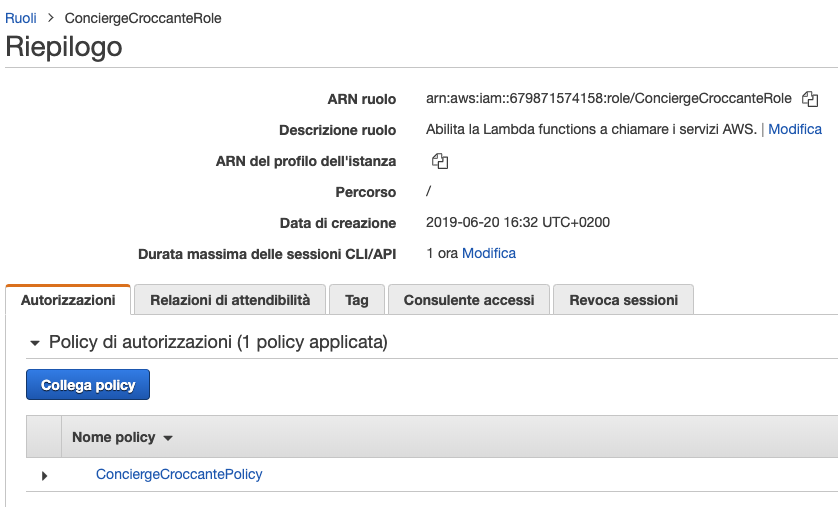
\includegraphics[width=1\columnwidth]{immagini/amazon-iam-role.png}
    \caption{\label{fig:esempio-amazon-iam-role}Esempio di Role creata}
\end{figure}

\newpage
\subsection{AWS CloudWatch}
Amazon CloudWatch\footnote{AWS CloudWatch. URL: \href{https://aws.amazon.com/it/cloudwatch/}{https://aws.amazon.com/it/cloudwatch/}} è un servizio di monitoraggio pensato per gli sviluppatori per fornire dati e analisi dal monitoraggio delle applicazioni, così da rispondere ai cambiamenti di prestazioni a livello di sistema, ottimizzare l'utilizzo delle risorse e ottenere una visualizzazione unificata dello stato di integrità operativa. CloudWatch raccoglie i dati di monitoraggio sotto forma di log, parametri ed eventi, unificando la loro visualizzazione, sulle applicazioni e i servizi eseguiti in AWS. Nel caso del progetto Concierce Croccante CloudWatch è stato utilizzato per rilevare comportamenti anomali della Skill, rilevando gli eventuali errori presenti nei log.
\begin{figure}[H] 
    \centering 
    
\includegraphics[width=0.8\columnwidth]{immagini/amazon-cloudwatch.png}
    \caption{\label{fig:icona_aws_cloudwatch}Icona AWS CloudWatch}
\end{figure}
\noindent Nel punto precedente, ovvero nel paragrafo \hyperref[aws-iam]{3.2.3}, è stato eseguito il procedimento necessario perché il servizio di CloudWatch venga abilitato. Pertanto non è necessario alcuna configurazione. Basterà recarsi al sito per poter utilizzare il servizio qualora si voglia visualizzare i dati sotto forma di log dopo o durante l'esecuzione di un servizio AWS, nel caso del progetto il servizio di AWS Lambda.

\subsection{AWS DynamoDB}
Amazon DynamoDB\footnote{AWS DynamoDB. URL: \href{https://aws.amazon.com/it/dynamodb/}{https://aws.amazon.com/it/dynamodb/}} è un servizio di database NoSQL (database non relazionale) proprietario e completamente gestito che supporta strutture di dati di tipo documento e di tipo chiave-valore. Caratteristiche di pregio sono database durevoli, multiregione e offrono sicurezza, backup, ripristino e cache in memoria per le applicazioni Internet. DynamoDB può gestire oltre 10 trilioni di richieste al giorno e supportando picchi di oltre 20 milioni di richieste al secondo. Nel progetto La Skill realizzata utilizza tale servizio per interrogare un database contenente la lista dei nomi del personale Crispy Bacon. 
\begin{figure}[H] 
    \centering 
    
\includegraphics[width=0.8\columnwidth]{immagini/amazon-dynamodb.png}
    \caption{\label{fig:icona_aws_dynamo}Icona AWS DynamoDB}
\end{figure}
\noindent È necessario quindi impostare tale servizio. Per farlo occorre recarsi nella pagina dedicata del db e una volta eseguito l'accesso con le proprie credenziali seguire le seguenti istruzioni:
\begin{itemize}
	\item Nel pannello a sinistra andare sulla sezione \texttt{Tabelle} e successivamente su \texttt{Crea Tabella};
	\item Nella nuova pagina sarà possibile settare le impostazioni della nuova tabella, quindi inserire un nome e due chiavi primarie, una di partizione e una di ordinamento, come mostra l'immagine seguente:
	\begin{figure}[H] 
        \centering 
        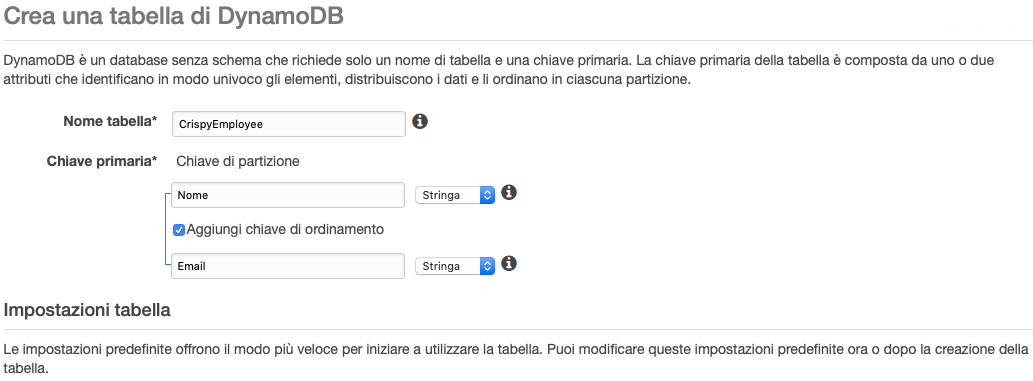
\includegraphics[width=1\columnwidth]{immagini/aws_dynamo.png}
	    \caption{\label{fig:esempio_aws_dynamo}Esempio creazione tabella AWS DynamoDB}
    \end{figure}
	
	\item Infine cliccare su \texttt{Crea}.
\end{itemize}
Ora è possibile popolare il database inserendo i dati nell'apposito pannello di controllo di DynamoDB oppure fare delle interrogazioni da codice.

\newpage
\section{Creazione della Skill}
Una volta configurati correttamente tutti i servizi di AWS che Concierge Croccante andrà ad utilizzare si è proceduti con la realizzazione vera e propria della Skill. In questa parte infatti si andrà a mostrare e spiegare come questa sia stata realizzata basandosi sull'analisi della VUI fatta al punto \hyperref[vui]{2.5}. Il processo di realizzazione della Skill parte dalla console per sviluppatori di Alexa, a seguire la creazione della funzione Lambda dove verrà eseguito il programma, terminando infine con la stesura del codice mostrando parti di esso ritenute fondamentali. 
\subsection{Alexa Developer Console}
Per creare la Skill C.C. è necessario visitare ed entrare nella console di gestione ed accedere al servizio Alexa Skills Kit\footnote{Alexa Skill Kit. URL: \href{https://developer.amazon.com/it/alexa-skills-kit}{https://developer.amazon.com/it/alexa-skills-kit}}. Una volta fatto l’accesso con le proprie credenziali si è proceduto a creare il prodotto:
\begin{itemize}
	\item Cliccare su \texttt{Create Skill} per creare la Skill;\\
	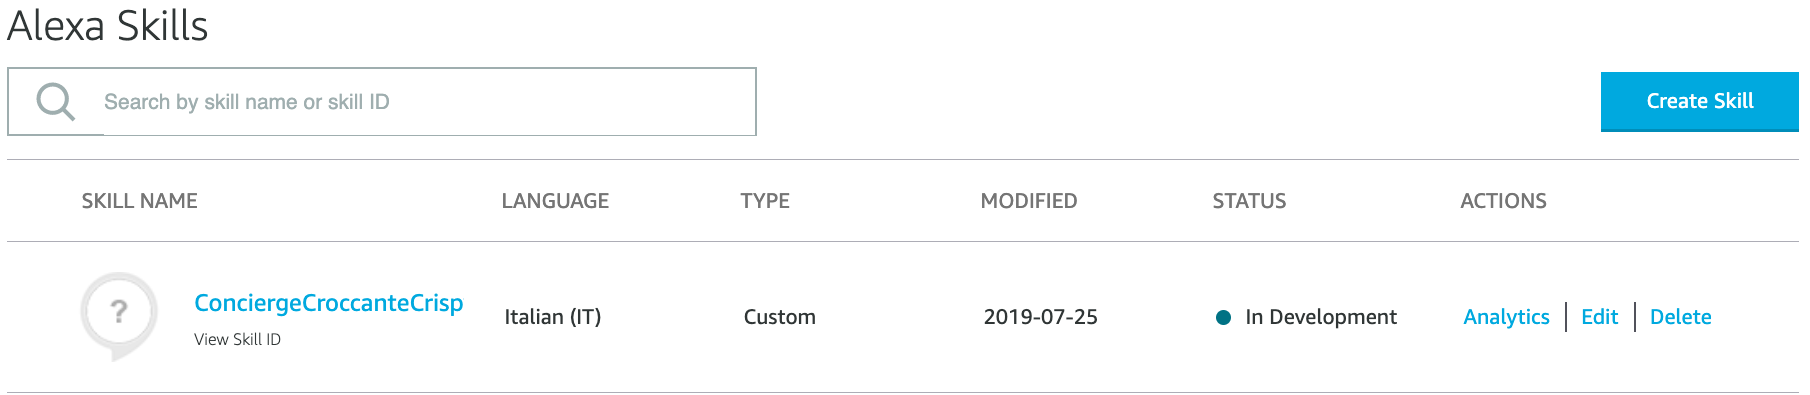
\includegraphics[width=12.5cm]{immagini/alexa-console-dev1.png}
	\item Nella pagina successiva, dare un nome alla propria Skill (facendo attenzione al fatto che quest'ultimo \textbf{non} sarà il nome di invocazione), scegliere la lingua, in questo caso \textit{Italian (IT)}, e scegliere \textit{Custom} come modello lasciando invariato il resto dei parametri. Successivamente cliccare nuovamente su \texttt{Create Skill};\\
	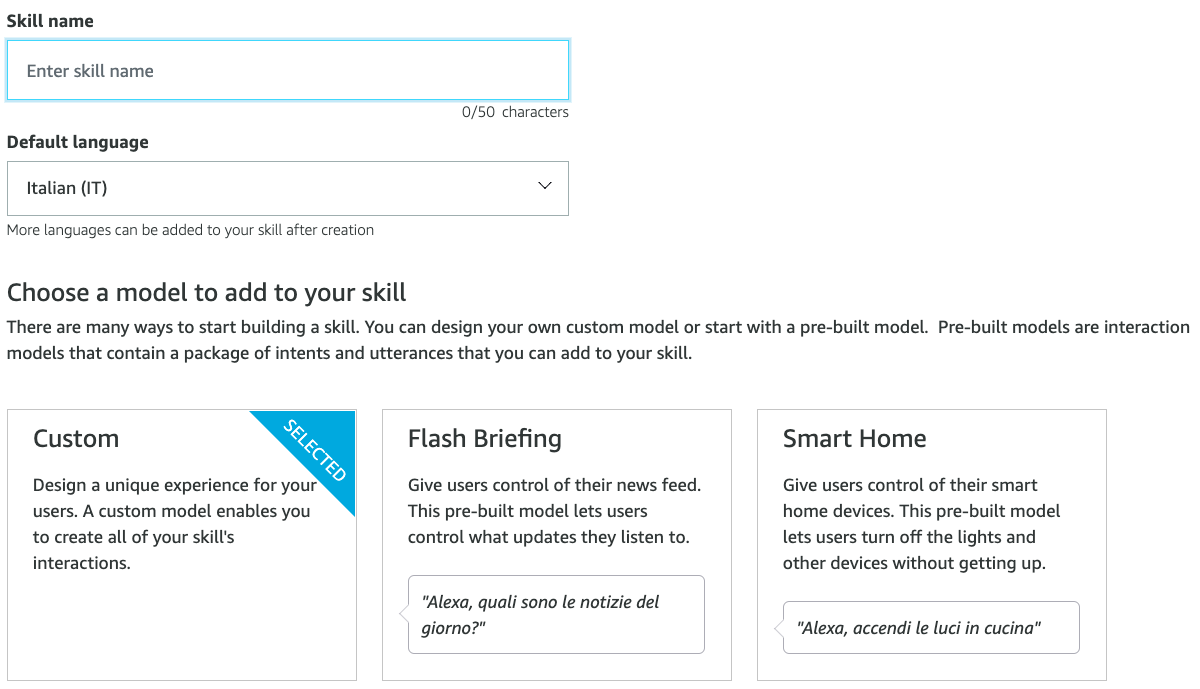
\includegraphics[width=13cm]{immagini/alexa-console-dev2.png}\\
	% 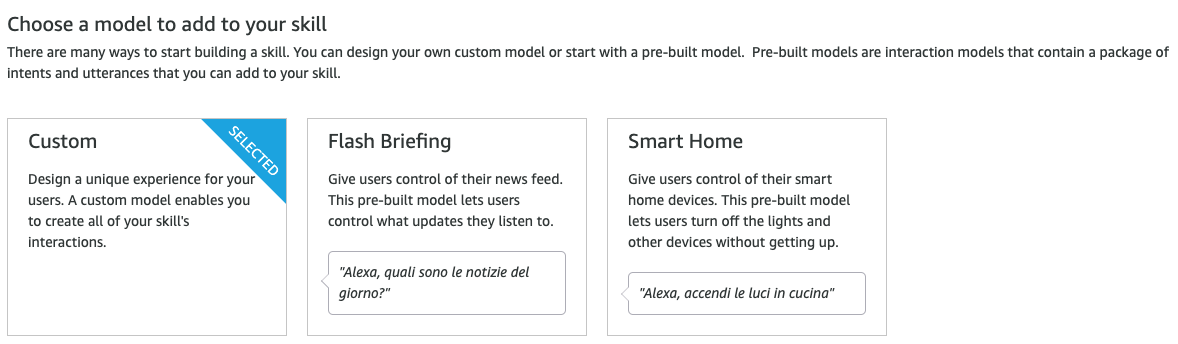
\includegraphics[width=12cm]{immagini/alexa-console-dev3.png}
	\newpage
	\item Si verrà reindirizzati nella pagina Alexa Developer Console dove sarà possibile customizzare la Skill. Nella sezione \texttt{Custom}, situata a sinistra, andare su \texttt{Invocation} per inserire il nome con cui si desidera invocare la Skill;\\[0.5cm]
	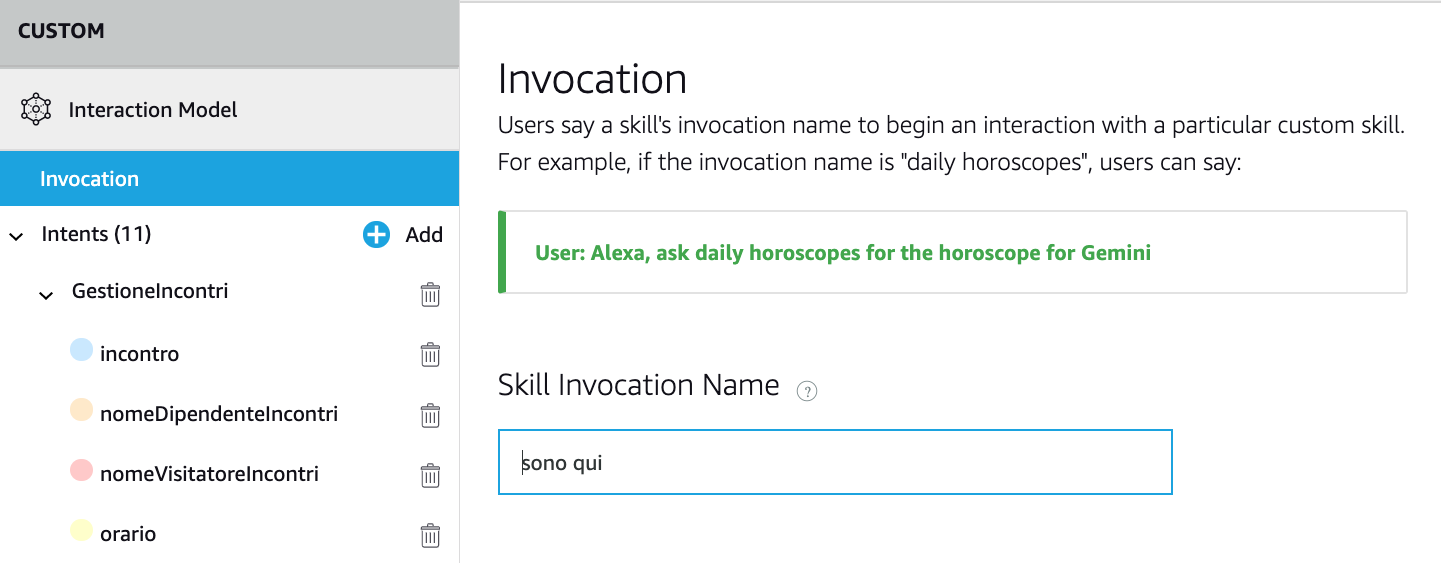
\includegraphics[width=12.5cm]{immagini/alexa-console-dev4.png}
	\item Successivamente è necessario creare gli intenti (\textit{intents}), che rappresentano un’azione che soddisfa una richiesta dell'utente. Sempre nella sezione \texttt{Custom} - \texttt{JSON Editor} è possibile creare gli intenti caricando un file .json oppure scrivendoli sull'editor della pagina. A questo punto il comando di invocazione e gli intents sono stati impostati correttamente.\\[0.5cm]
	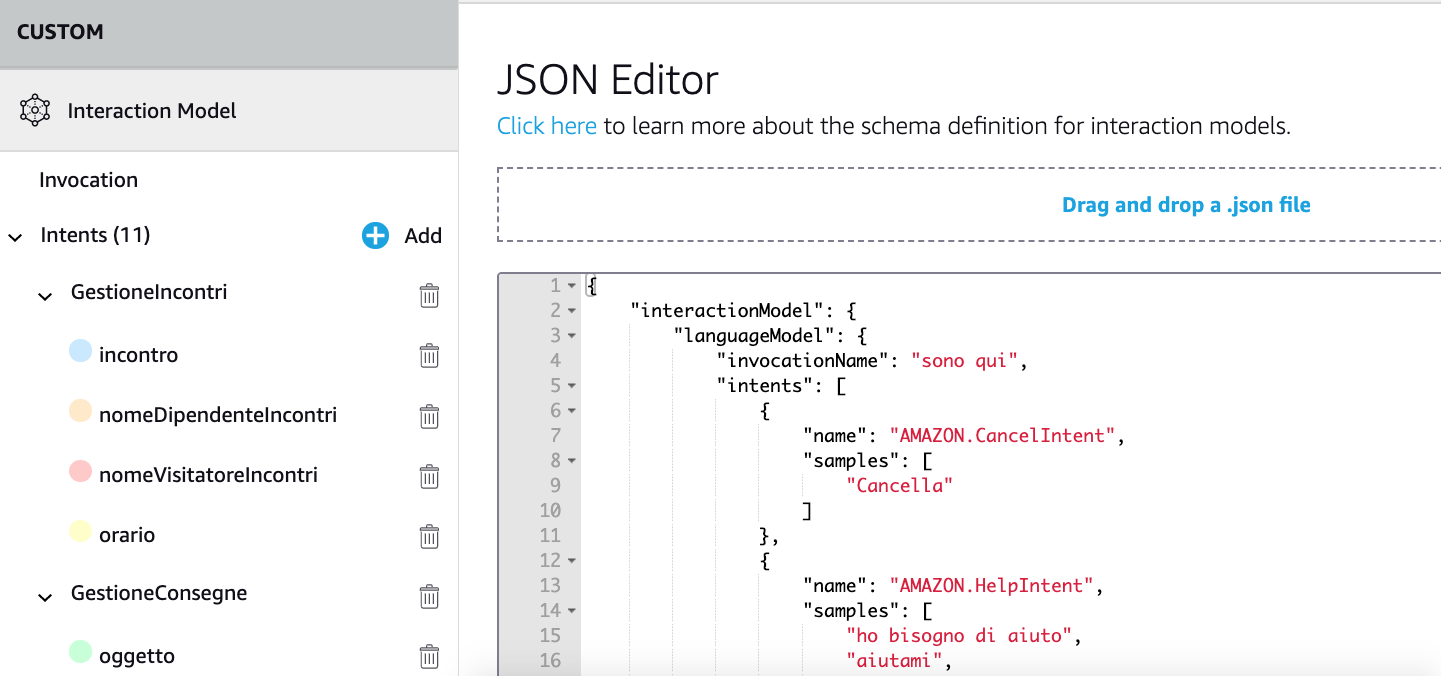
\includegraphics[width=12.5cm]{immagini/alexa-console-dev5.png}
\end{itemize}

\newpage
\noindent \subsubsection{Skill ID}
Il passo seguente è stato quello di salvare lo Skill ID, la chiave identificativa della Skill appena creata, che nei passi successi servirà per impostare l'endpoint: ovvero collegare la Skill alla Lambda dove risiederà il codice. Per fare ciò è stato sufficiente identificare e salvare l'ID inglobato nell'indirizzo URL della Skill appena creata, come mostra l'immagine seguente:
\begin{figure}[H]
	\centering
	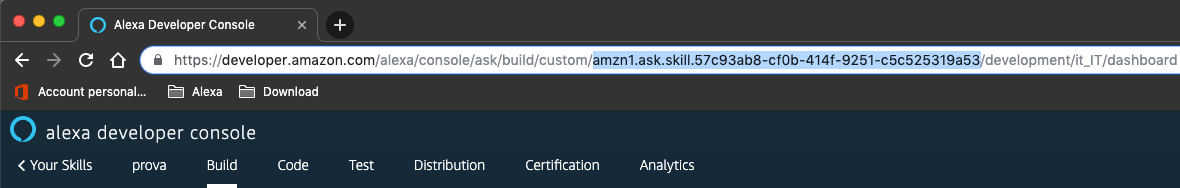
\includegraphics[width=13cm]{immagini/url_skill.png}
	\caption{Esempio Skill ID}
\end{figure}

\subsection{AWS Lambda}
Amazon Lambda\footnote{AWS Lamba. URL: \href{https://aws.amazon.com/it/lambda/}{https://aws.amazon.com/it/lambda/}} è un servizio della suite AWS che consente di eseguire codice senza dover effettuare il provisioning\footnote{In telecomunicazioni è un servizio cloud a disposizione dell'utente che include hardware, software, cablaggio ed altro} e gestire server. Con Amazon Lambda è quindi possibile eseguire codice per qualsiasi tipo di applicazione o servizio back-end, senza alcuna amministrazione. Caricato il codice, Lambda attua tutte le azioni necessarie per eseguirlo e ricalibrare le risorse con massima disponibilità. È possibile anche configurare il codice in modo che venga attivato automaticamente da altri servizi AWS oppure che venga richiamato direttamente da qualsiasi applicazione Web o mobile.\\[0.5cm]
Una volta proceduti a creare la Skill la fase successiva è stata la realizzazione della funzione Lambda necessario per l'esecuzione del codice C.C.. Recandosi nell'omonima pagina, Amazon Lambda, sono stati eseguiti i passaggi di configurazione per creare la funzione ospitante il codice implementato o in fase di implementazione. Una volta fatto l'accesso con le proprie credenziali si è proceduto nel seguente modo:
\begin{minipage}{0.5\textwidth}
	\begin{figure}[H]
		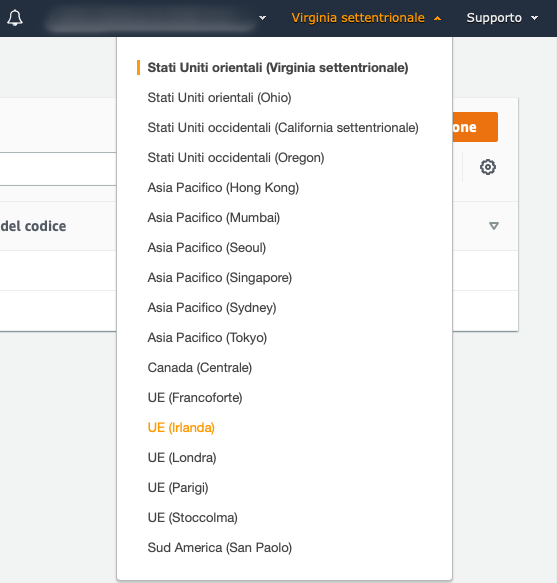
\includegraphics[width=6cm]{immagini/aws-lambda.png}
		\caption{\label{fig:aws_lambda_regione}Selezione regione AWS Lambda}
	\end{figure}
\end{minipage}
\begin{minipage}{0.5\textwidth}
	Prima di procedere è importate cambiare la regione di esecuzione della funzione Lambda. Quindi cliccare in alto a destra sulla regione (seconda voce) e scegliere \textit{UE (Irlanda)}, come mostrato in figura. Questo passaggio è necessario perché in base alla regione scelta, AWS - Lambda mette a disposizione più o meno servizi da integrare con la funzione. Tali informazioni possono essere reperite nell'apposita pagina\footnote{Servizi per regioni. URL: \href{https://amzn.to/30GkmTd}{https://amzn.to/30GkmTd}}. Di seguito viene fornito anche URL delle \href{https://amzn.to/2NCexm7}{Regioni ed endpoint AWS}\footnote{Endpoint AWS. URL: \href{https://amzn.to/2NCexm7}{https://amzn.to/2NCexm7}} dove sono riportate le informazioni degli endpoint di ogni servizio per ciascuna regione.
\end{minipage}
\begin{itemize}
	\item Cliccare in alto a destra su \texttt{Crea funzione} per creare la Lambda;
	\item Nella pagina successiva, dare un nome alla funzione su cui verrà caricato il codice, nella sezione \texttt{runtime} scegliere \textit{Node.js 10.x} e infine nella sezione \texttt{Autorizzazioni} - \texttt{Ruolo di esecuzione} scegliere \textit{Utilizza ruolo esistente - ConciergeCroccanteRole} (ruole creato in precedenza durante la configurazione di AWS IAM al punto \hyperref[aws-iam]{3.2.3}). L'immagine seguente mostra la scelta corretta delle impostazioni base;\\[0.3cm]
	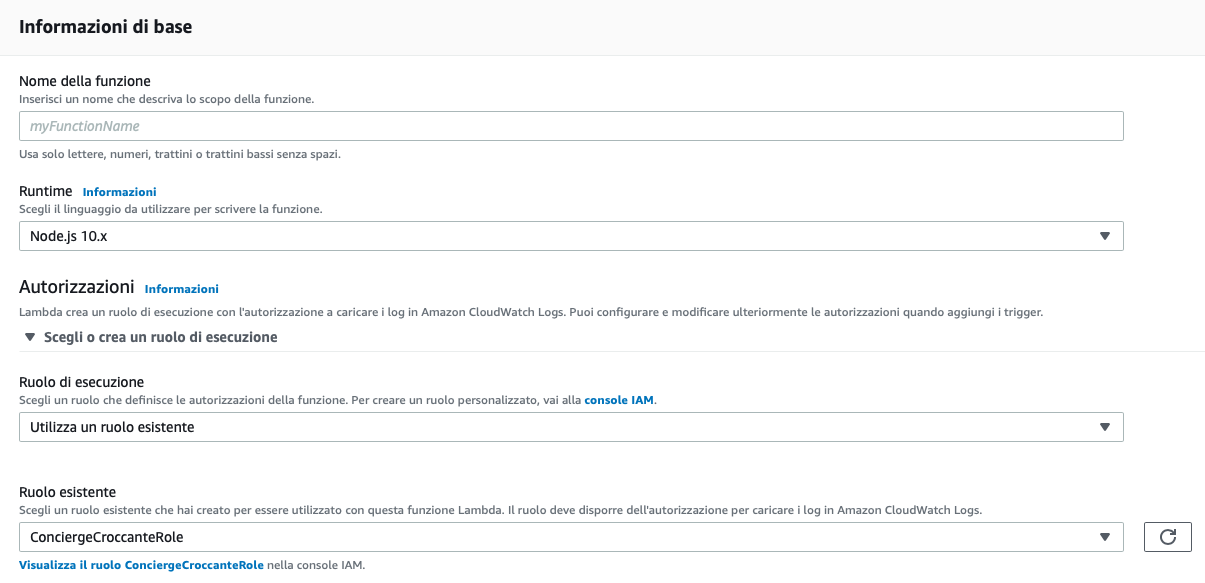
\includegraphics[width=13cm]{immagini/aws-lambda2}
	\item Successivamente cliccare nuovamente su \texttt{Crea funzione};
	\item Ora la funzione è stata impostata con le autorizzazioni sufficienti e necessarie per poter utilizzare i servizi che la Skill necessita. A destra cliccare su \texttt{Aggiungi trigger}, selezionare \texttt{Alexa Skill Kit}, inserire la Skill ID (salvata in precedenza) e cliccare su \texttt{Aggiungi}.
\end{itemize}
\subsubsection{Endpoint}
\label{endpoint}
Ora è possibile terminare il processo di configurazione della Skill eseguendo il collegamento tra Skill e Lambda. Ritornando nella console di AWS, sul servizio Lambda, è stato copiato l'indirizzo ARN della funzione, situato in alto a destra, come mostra nell'immagine seguente:
\begin{figure}[H]
	\centering
	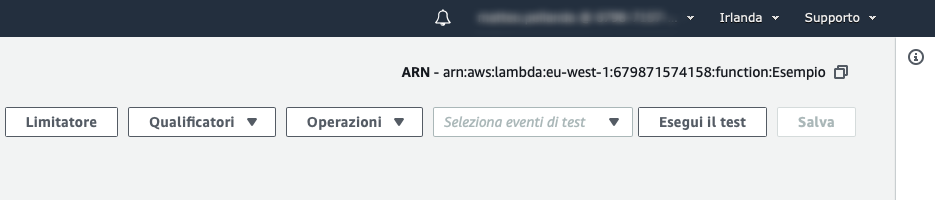
\includegraphics[width=13cm]{immagini/aws-lambda3.png}
	\caption{Esempio URL ARN Lambda}
\end{figure}
\noindent Successivamente, nella Skill in Alexa Developer Console, nella sezione \texttt{Custom} - \texttt{Endpoint}, incollare l'URL ARN della Lambda copiato in \texttt{Default Region}.
\begin{figure}[H]
	\centering
	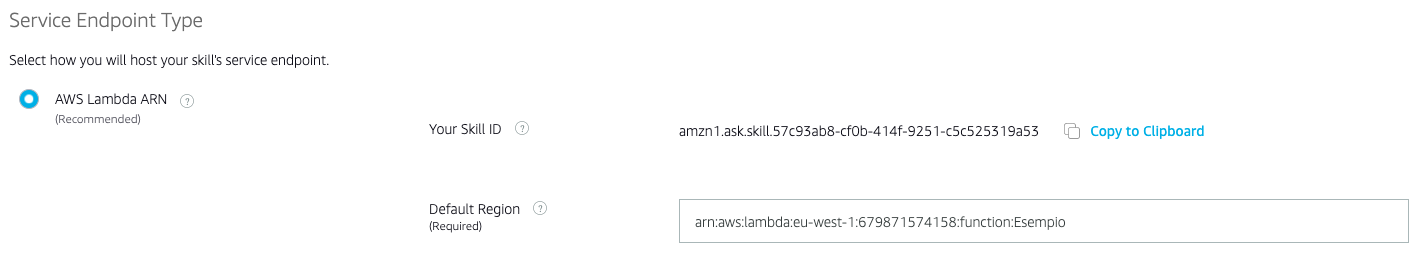
\includegraphics[width=13cm]{immagini/aws-lambda4.png}
	\caption{Esempio URL ARN Lambda}
\end{figure}
\noindent Infine cliccare su \texttt{Save Endpoint}. Ora la Skill l'endpoint impostato con l'esecuzione della funzione lambda creata.\\
Non rimane altro che caricare il codice del prodotto. Per farlo basterà recarsi nuovamente sulla console di AWS nel servizio Lambda, scegliere la propria funzione e su \texttt{Codice della funzione} scegliere \textit{Carica un file .zip} per caricare la cartella compressa del progetto.
\begin{figure}[H]
	\centering
	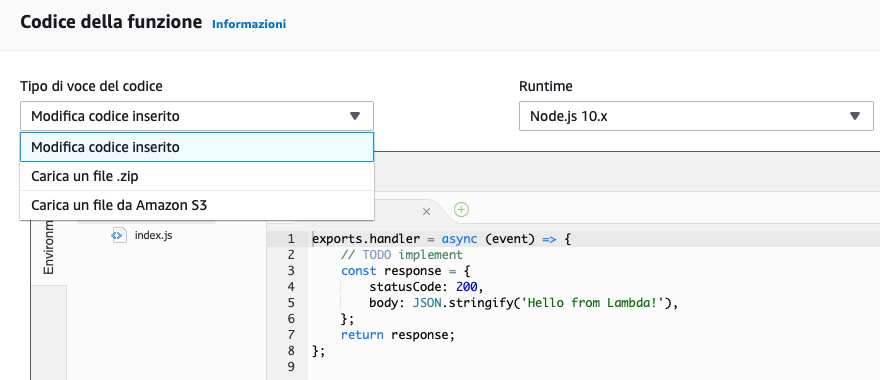
\includegraphics[width=13cm]{immagini/aws-lambda5.png}
	\caption{Codice funzione}
\end{figure}



